\chapter{Stos protokołów LTE}
\label{cha:protokoly}

Protokoły stosowane w systemach LTE możemy podzielić na 2 grupy: protokoły płaszczyzny użytkownika oraz protokoły płaszczyzny kontroli.

Protokoły płaszczyzny użytkownika (Rys. \ref{fig:userPlaneProtocols}) odpowiedzialne są za przesył danych użytkownika dostarczanych przez wyższe warstwy, np. przez warstwę Internet Protocol (IP). Natomiast protokoły płaszczyzny kontrolnej (Rys. \ref{fig:controlPlaneProtocols}) są odpowiedzialne za zarządzanie połączeniem poprzez konfigurację poszczególnych warstw płaszczyzny użytkownika lub zarządzanie zasobami radiowymi.

\begin{figure}
	\centering
		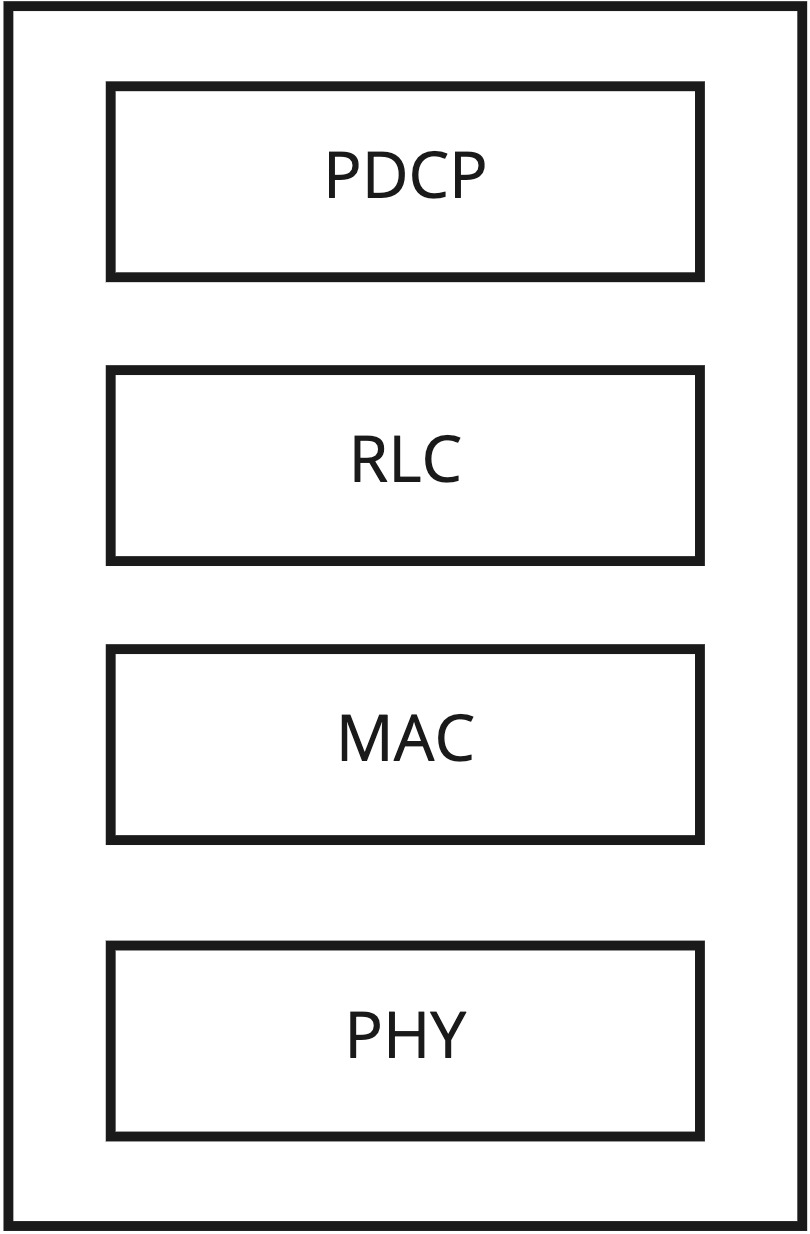
\includegraphics[width=0.2\textwidth]{user-plane-protocols.jpg}
	\caption{Stos protokołów dla płaszczyzny użytkownika}
	\label{fig:userPlaneProtocols}
\end{figure}


\begin{figure}
	\centering
		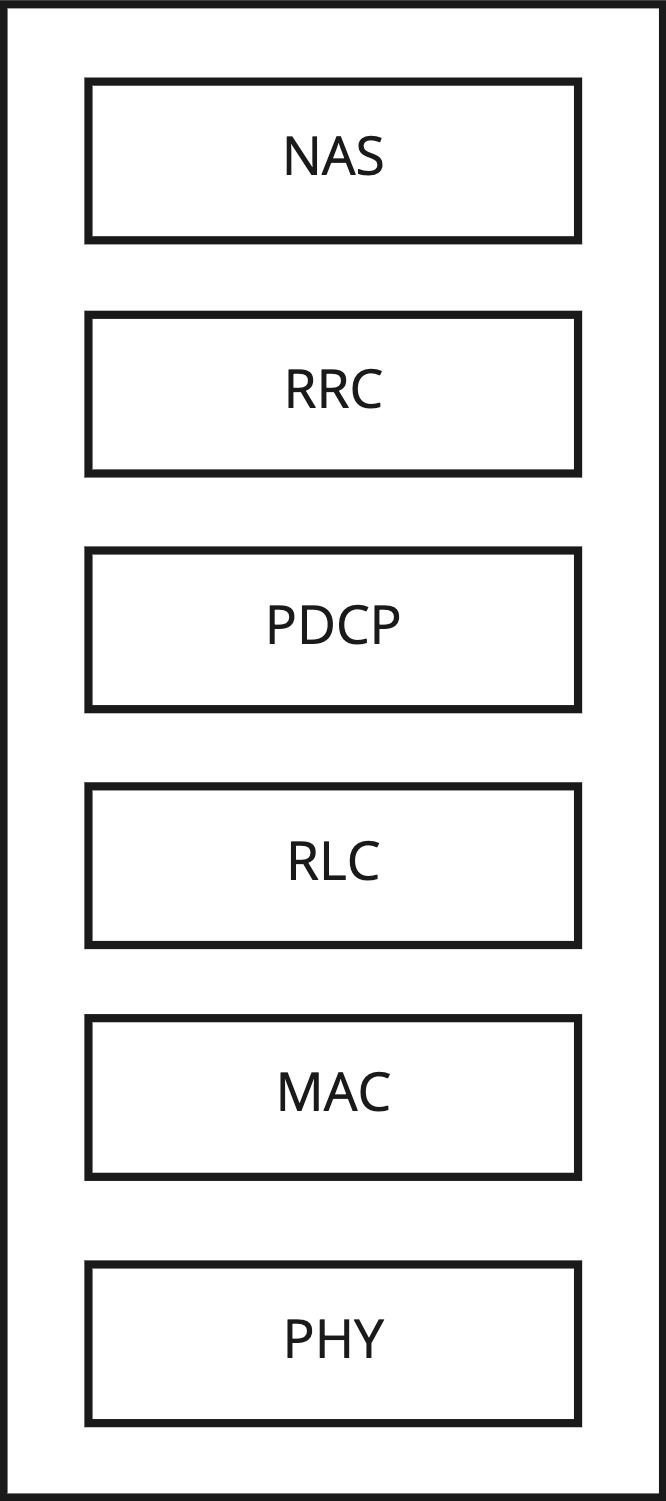
\includegraphics[width=0.2\textwidth]{control-plane-protocols.jpg}
	\caption{Stos protokołów dla płaszczyzny kontrolnej}
	\label{fig:controlPlaneProtocols}
\end{figure}

